\documentclass[12pt]{exam}

\usepackage{graphicx} % allows for graphics
\usepackage{ifthen}  % for if statements 

\newcommand{\sol}{1} %solution =1 or 0

% LOAD PACKAGES
\usepackage{amsmath} % allows for align env and other things
\usepackage{amssymb} % 
\usepackage{mathtools} % allows for single apostrophe
\usepackage{enumitem} % allows for alpha lettering in enumerated lists
\usepackage{lastpage}
\usepackage{array} % for table alignments
\usepackage{graphicx} % if images are needed

\addpoints

\usepackage{pgfplots} % for surfaces (chapter 7)
\usepackage{tikz-3dplot} 
\pgfplotsset{compat=1.9}
\usetikzlibrary{decorations.pathmorphing,patterns} % for some tikz diagrams
% ~~~~~~~~~~~~~~~~~~~~~~~~~~~~~~~~~~~~
% INITIALS
\newcommand{\Initials}{\textit{\Course, \TestName. Your initials: \underline{\hspace{3cm}}} \vspace{1pt}}

\newcommand{\InitialsLeft}{\noindent \hspace{-18pt}\textit{\Course, \TestName. Your initials: \underline{\hspace{3cm}}} \vspace{1pt}}

\newcommand{\InitialsRight}{\begin{flushright}\textit{\Course, \TestName. Your initials: \underline{\hspace{3cm}}} \vspace{1pt}\end{flushright}}

% ~~~~~~~~~~~~~~~~~~~~~~~~~~~~~~~~~~~~
% INSTRUCTIONS FOR DISTANCE LEARNING WITH NO PROCTOR
\newcommand{\InstructionsFormatAndTiming}{

    \begin{itemize} \setlength\itemsep{.1em}
    
        % \item You should only need 75 min to take the exam, but students will have \Duration to submit the exam, from the time that it is released.
        
        \item {\bf Show your work} and justify your answers for all questions unless stated otherwise.
        
        \item Please write neatly, and use dark and clear writing so that the scan is easy to read. 
        
        \item Please write your name or initials at the top of every page 
        
        \item Please solve the questions in the exam in the order they are given. 
        
        \item You do not need to print the exam. As long as you solve problems in the order they are given (just like the written homework sets), you can write your answers on your own paper. But students can print the exam and write their answers on the printed copy if they prefer. 
        
    \end{itemize}

}

\newcommand{\InstructionsSubmission}{

    \begin{itemize} \setlength\itemsep{.1em}
        \item Students should scan their work and submit it through Gradescope. There should be an \textbf{assignment} in Gradescope for this exam. The process for submitting your work will be similar to what you have used for homework. 
        
        \item Work must be submitted by \DueDate. 
        
        \item Please upload your work as a single PDF file. If this is not possible you can email your work to your instructor. 
        
        \item During the upload process in Gradescope, please indicate which page of your work corresponds to each question in the exam. 
    \end{itemize}
}

\newcommand{\InstructionsQuestions}{

    \begin{itemize} \setlength\itemsep{.1em}
        
        \item If there are questions during the exam, students can email their instructor or message them through Canvas. 
        
        \item Our course Piazza forum will be temporarily inactive during the exam. 
        
        \item If you run into any technical issues or any unanticipated emergencies, please email your instructor as soon as you can. 
    
        
    \end{itemize}

}


\newcommand{\InstructionsHonor}{

    \begin{itemize} \setlength\itemsep{.1em}    
        \item Students can use any resources while taking these tests including online calculators and Mathematica
        \item Students cannot communicate with anyone during these tests.
        \item Students cannot use solutions provided from another student or third party. 
        \item In other words: do your own work but you can use technology to solve problems. 
 
    \end{itemize}

}






\newcommand{\GTHonorCode}{Having read the Georgia Institute of Technology Academic Honor Code, I understand and accept my responsibility as a member of the Georgia Tech community to uphold the Honor Code at all times. }



% FANCY HEADERS - MAKE EMPTY
\pagestyle{headandfoot}
\runningfooter{}{}{}


% ADJUST MARGINS FOR DISTANCE LEARNING REQUIREMENTS
\usepackage[tmargin=1.0in,bmargin=1.0in,left=1in,right=1in]{geometry}


% TIKZ DIAGRAMS
\usepackage{color}
\usepackage{tikz}  \usetikzlibrary{arrows} 
\usetikzlibrary{calc} 


% ADJUST FIRST LINE IN PARAGRAPH INDENTATION 
\setlength\parindent{0pt}


% COURSE SPECIFIC INFORMATION
\newcommand{\Course}{Math 2552}
\newcommand{\Instructors}{}

% WHO TO CONTACT DURING EXAM IF QUESTIONS
\newcommand{\InstructorContact}{}

\usepackage{spalign} % Joe Rabinoff's matrix package

\newcommand{\LastPage}{\begin{center}\textit{This page may be used for scratch work. Please indicate clearly if you would like your work on this page to be graded. }\end{center}   }


% DERIVATIVES
\newcommand{\dydt}{{\frac{dy}{dt}}} % 
\newcommand{\dydx}{{\frac{dy}{dx}}} % 
\newcommand{\dydtt}{{\frac{d ^2y}{dt^2}}} % 
\newcommand{\dydxx}{{\frac{d^2y}{dx^2}}} % 
\newcommand{\dydttt}{{\frac{d^3y}{dt^3}}} % 

\newcommand{\ddt}{{\frac{d}{dt}}} % 
\newcommand{\ddx}{{\frac{d}{dx}}} % 
\newcommand{\dudt}{{\frac{du}{dt}}} % 
\newcommand{\dvdx}{{\frac{dv}{dx}}} % 
\newcommand{\dxdt}{{\frac{dx}{dt}}} % 
\newcommand{\dxdtt}{{\frac{d^2x}{dt^2}}} % 
\newcommand{\dzdt}{{\frac{dz}{dt}}} % 



% COLORS FOR DIAGRAMS
\definecolor{DarkBlue}{rgb}{0.0,0.0,0.6} % 
% \definecolor{DarkGreen}{rgb}{0.0,0.3,0.0} % 
% \definecolor{DarkRed}{rgb}{0.6,0.0,0.0} % 

% TEST SPECIFIC INFORMATION
\newcommand{\TestName}{Sample Midterm 2}
\newcommand{\TestTime}{}
\newcommand{\Duration}{3 hours }
\newcommand{\Points}{}
\newcommand{\DueDate}{12:30 PM ET}


% \usepackage{tikz}
% \usetikzlibrary{shapes,snakes}   
% \usetikzlibrary{arrows,automata}

\begin{document}
    

\vspace*{-1cm}

\begin{center}
{\Large \TestName, \Course }
\end{center}

% \begin{center}    
% {\small
% Instructor: \Instructors \\ Administered on \TestDate. Students should have 3 hours to take this exam. 
% }
% \end{center}


% INSTRUCTIONS FOR STUDENTS
\vspace{2pt}
\begin{center}\textbf{{\large Instructions (PLEASE READ)}}\end{center}
\textbf{Formatting and Timing}
{\small \InstructionsFormatAndTiming}
\textbf{Submission}
{\small \InstructionsSubmission}
\textbf{Questions}
{\small \InstructionsQuestions}
\textbf{Integrity}
{\small \InstructionsHonor}

 % cover page for unproctored exam

\newpage


\begin{questions}


    \question[10]  Solve the differential equation. $$y''+y = \sec x$$
    You may find the formula $$\int \tan x \, dx = - \ln |\cos x|$$ helpful. 
    \newpage

        \question[9] Consider a lattice with $3$ lattice points, as in the figure below. 
    
        \begin{center}
            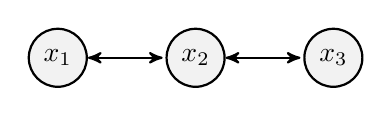
\begin{tikzpicture}
                \begin{scope}[<->,>=stealth',shorten >=1pt,auto,node distance=1.75cm,thick, main node/.style={circle,fill=gray!10,draw}]
                \node[main node] (1) {$x_1$};
                \node[main node] (2) [right of=1] {$x_2$};
                \node[main node] (3) [right of=2] {$x_3$};
                \path[every node/.style={font=\sffamily\small}]
                (1) edge node[below] {} (2)
                (2) edge node [above] {} (3);
                \end{scope}
            \end{tikzpicture}  
        \end{center}  
        
        Let $x_j(t)$ be the number of particles residing at the $j$th lattice point at time $t \ge 0$. Assume that $x_j$ satisfies the following rate equations.
        \begin{align*} 
            \frac{dx_1(t)}{dt} = x_2 - x_1 , \qquad 
            \frac{dx_2(t)}{dt} = x_3 - 2 x_2 + x_1 , \qquad \frac{dx_3(t)}{dt} = x_2 - x_3
        \end{align*} 
        % Answer the following questions.
        \begin{enumerate} 
            \item[a)] Express the system of equations in the form $\vec x \, ' = A \vec x$. 
                \vspace{2cm}

                \item[b)] Determine the eigenvectors of $A$ and write down the general solution. You may use that the eigenvalues of $A$ are $0, -1$ and $-3$. 
                \vspace{10cm} 
                \item[c)] What does the solution converge to as $t \to \infty$? 
        \end{enumerate}


    % \question[10] Solve the initial value problem. 
    % $$\vec x \, ' = \frac 1 2 \spalignmat{-2 -1;1 0} \vec x, \quad \vec x (0) = \spalignmat{-1 ;0}$$

    \newpage
    
    \question[8] Solve the differential equation using the method of undetermined \\coefficients. $$y'' + 4y = 3 \sin(2t)$$
    

    \newpage 
    

    \vspace{4cm} 
    
    \question[8] The position of a moving object, $y(t)$, satisfies the IVP $$y''+2y'+5y=0, \quad y(0) = 0, \quad y'(0) = 4$$ The solution is $y(t)= 2e^{-t}\sin(2t)$. 
    
    \begin{parts} 
        \part Give a rough sketch of the solution, $y(t)$ for $t>0$. Label your axes.\vspace{4cm}
        \part For $t \ge 0$, sketch the trajectory of the object in the phase plane. Indicate the location corresponding to $t=0$, the direction of motion, and label your axes.  
        
    \end{parts}
    
    \newpage
    \question[4]  Construct an initial value problem for the following situation. 

    \begin{itemize}
        \item[] A spring is stretched 0.5 m by a force of 0.25 newtons (N). A mass weighing 2 kg is attached to a spring that is also attached to a viscous damper that applies a force of 10 N when the velocity of the mass is 5 m/s. The mass is pulled down 2 m below its equilibrium position and given an initial upward velocity of 4 m/s. 
    \end{itemize}
    
    \vspace{4cm} 
    
    \question[3] If $W[f, g]$ is the Wronskian of $f$ and $g$, and if $u=2f - g, \ v=f +2g$, find the Wronskian $W[u,v]$ of $u$ and $v$ in terms of $W [ f , g]$.

    \vspace{6cm} 
    
    \newpage
    
    \question[8] Use the method of reduction of order to find a second solution $y_2$ of the given differential equation such that $\{y_1, y_2\}$ is a fundamental set of solutions on the given interval. $$t^2y'' - t(t+2)y' + (t+2)y=0, \quad t > 0 , \quad y_1(t) = t$$
    
        
\end{questions}



\newpage

\large{Answers}

\begin{enumerate}

\item[5)] Using $mg = kL$, $0.25 = \frac 12 k$, so $k = 1/2$. Damping: \begin{align*}F_d &= \gamma v \\ 10&=5 \gamma  \\
\gamma &= 2\end{align*}
DE and conditions give the IVP: 
$$2y'' +2y' + \frac 12 y = 0, \quad y(0) = 2, \quad y'(0) = -4$$ 
\item[6)] This is 4.2 \# 20. $W(f,g) = fg' - f'g$. Also, $W(u,v) = W(2f - g,f + 2g) $. Then, $W(u,v) =(2f-g)(f+2g)'
 - (2f- g)'(f+2g)= 5fg' - 5f'g = 5W(f,g)$. 

\item[7)] This is 4.2 \# 32. Let $y_2(t) = tv(t)$. 

$$y_2' = v + tv', \quad y'' = 2v' + tv''$$

Substituting $y$ into the differential equation, we obtain 
\begin{align*}
    0 &= t^2y'' - t(t+2)y' + (t+2)y \\
    &= t^2(2v' + tv'') - t(t+2)(v + tv') + (t+2)tv \\
    &= (t^3v'' +2t^2v') - ( t^2v + t^3v' + 2tv + 2t^3v') + (t^2v+2tv) \\
    &= t^3v'' - t^3 v' \\
    &= v'' - v'
\end{align*}
This is a separable (and linear) DE. 
\begin{align*}
    v'(t) &= ce^t \\
    v(t) &= c_1 e^t + c_2 \\
    y_2(t) &= tv(t) = c_1te^t + c_2t
\end{align*}

Since we already have $y_1(t) = t$, we do not need the $c_2t$ term (we only need two independent functions to form a fundamental set). So we are free to set $c_1 = 1$ and $c_2 = 0$. Therefore, we get the solution $y_2(t) = te^t$. \\[12pt] \textit{Note that it would not be wrong to leave the $c_2t$ term in the solution, but a more succinct solution would be obtained if we set $c_2 = 0$. }
\end{enumerate} 


\end{document}